\documentclass[12pt,a4paper]{article}
\usepackage{tikz}
\usetikzlibrary{arrows.meta,positioning}
\usepackage{tabularx}
\usepackage{graphicx}
\usepackage{amsmath}
\usepackage{amssymb}
\usepackage{amsthm}
\usepackage{bm}
\usepackage{hyperref}
\usepackage{booktabs}
\usepackage{array}
\usepackage{geometry}
\geometry{margin=2.5cm}
\hypersetup{colorlinks=true, linkcolor=blue, citecolor=blue, urlcolor=blue}

\title{\textbf{Paper E-01: Cross-Domain AFL Hypothesis Synthesis:\\ A Constraint-Driven Flux Dynamics (CDFD) Perspective}}
\author{Steve Bico Mujjabi, MD\\
\small Independent Researcher\\
\small Founder, Vura Labs\\
\small Kampala, Uganda\\
\small ORCID: 0009-0001-0556-5516}
\date{August 2026}

\begin{document}
\maketitle

% BEGIN SHARED-METHODS POINTER
\noindent\textit{Shared Part IV notation and evidence boundaries are defined in \path{PART_IV_METHODS_AND_CLAIM_BOUNDARY.md}. This paper states only its local observables, comparison, and failure conditions.}
% END SHARED-METHODS POINTER

\begin{abstract}
This synthesis states the common Part IV modelling relation and the release
boundary for cross-domain claims. Across Earth systems, engineered systems,
socioeconomic systems, domain applications, cosmic and subatomic systems, and
abstract or cognitive systems, CDFD/AFL uses the same candidate variables:
driving flux $\Phi$, constraint $C$, responsiveness $S$, and structural memory
$M_s$. Shared notation does not imply shared material mechanism or empirical
validation. The release-local runtime outputs are internal diagnostics and
tests that could break the mapping.
\end{abstract}
% BEGIN CONSOLIDATION SCOPE
\section*{Consolidation Scope and Provenance}
This synthesis now absorbs the family-level overviews formerly carried by Papers A-12, B-12, and C-10. It remains a claim-boundary and comparison document, not an additional empirical domain paper or a universal-law statement.
% END CONSOLIDATION SCOPE


\section{Series Context}

Part I sets the flow--constraint language used here \cite{MujjabiPartI2026}.
Part II develops the Life Number and the origins-of-life use of the same notation
\cite{MujjabiPartII2026}. Part III applies AFL to biology and medicine
\cite{MujjabiPartIII2026}. Part IV \cite{MujjabiPartIV2026}, DOI \url{https://doi.org/10.5281/zenodo.20395901}, extends the notation into a cross-domain
release archive and keeps claim status visible beside every synthesis claim.

\section{Common Relation}

Part IV uses the operating ratio
\begin{equation}
    \Psi_s^* = \left(\frac{\Phi}{C}\right) \cdot S \cdot M_s,
\end{equation}
with the reduced form $\Phi/C$ used only when $S=1$ and $M_s=1$. The companion
constraint-update form is
\begin{equation}
    \frac{\partial C}{\partial t} = \alpha |\Phi| - \beta C + \gamma \nabla^2 C.
\end{equation}

These equations are a modelling grammar. A domain claim becomes stronger only
when each term has a measurable proxy, a time scale, a spatial or network
scale, and a failure condition.

\section{Cross-Domain Reading}

The Part IV sections use the same form for different reasons:
\begin{itemize}
    \item Part A asks how environmental systems carry heat, water, matter, and
    biological throughput under constraint.
    \item Part B asks how engineered systems balance throughput against
    capacity, state, and responsiveness.
    \item Part C asks how social and economic systems accumulate memory,
    friction, and institutional constraint.
    \item Part D tests additional domain mappings, from immunology and
    population genetics to information flow.
    \item Part F applies the notation to cosmic and subatomic examples as
    hypothesis-level analogies.
    \item Part G treats language, science, and AI as cognitive or abstract
    transport systems.
\end{itemize}

\section{Measurement Layer}

\section{Current Runtime Diagnostic}

The release-local discovery script
produces a domain adapter sweep, a network-cascade stress test, two figures,
and a generated Markdown summary. The run records finite-value behavior and
overload/memory-locking dynamics in the current CDFD Runtime. It is a model
record for later measurement, not a claim that the domains have already been
validated.

\section{Claim Standard}

A Part IV claim is stronger when it names the measured $\Phi$, $C$, $S$, and
$M_s$ proxies; states the expected direction of change; gives the time and
network scale; identifies a dataset or experiment; and states what result would
falsify the CDFD/AFL interpretation.

\section{Boundary}

The cross-domain synthesis is not operational advice for infrastructure, finance,
medicine, climate intervention, AI safety, or policy. It is a modelling archive
with reproducible local diagnostics. Any applied use requires ordinary domain
validation and expert review.

% BEGIN PART IV MAJOR CROSS-DOMAIN UPGRADE
\section{Cross-Domain Model Upgrade: Mechanism, Scale, and Tests}

\subsection{Observable Translation}

The paper-specific translation begins with an observable chain rather than a
verbal analogy. For Universal AFL Synthesis, the proposed drive is domain-specific flows of energy, matter, information, organisms, capital, and force.
The active limitation is measured bottlenecks and finite capacities in each domain. Responsiveness is carried by
domain-specific adaptation, buffering, rerouting, repair, and control, while retained state is represented by
retained physical, biological, technical, institutional, or cognitive state. The outcome to explain is overload, transition, recovery, and comparative transfer.

\begin{table}[htbp]
\centering
\small
\caption{Operational CDFD/AFL map for Paper E-01.}
\begin{tabularx}{\textwidth}{|l|X|X|}
\hline
\textbf{Term} & \textbf{Paper-specific observable meaning} & \textbf{Measurement question} \\
\hline
$\Phi$ & domain-specific flows of energy, matter, information, organisms, capital, and force & What rate, load, gradient, or demand enters the focal system? \\
\hline
$C$ & measured bottlenecks and finite capacities in each domain & Which measured bottleneck limits transfer, function, or recovery? \\
\hline
$S$ & domain-specific adaptation, buffering, rerouting, repair, and control & Which process changes effective capacity or reroutes the load? \\
\hline
$M_s$ & retained physical, biological, technical, institutional, or cognitive state & Which retained state makes equal present loads produce different futures? \\
\hline
$Y$ & overload, transition, recovery, and comparative transfer & Which outcome is predicted out of sample, with uncertainty? \\
\hline
\end{tabularx}
\end{table}

\begin{figure}[htbp]
\centering
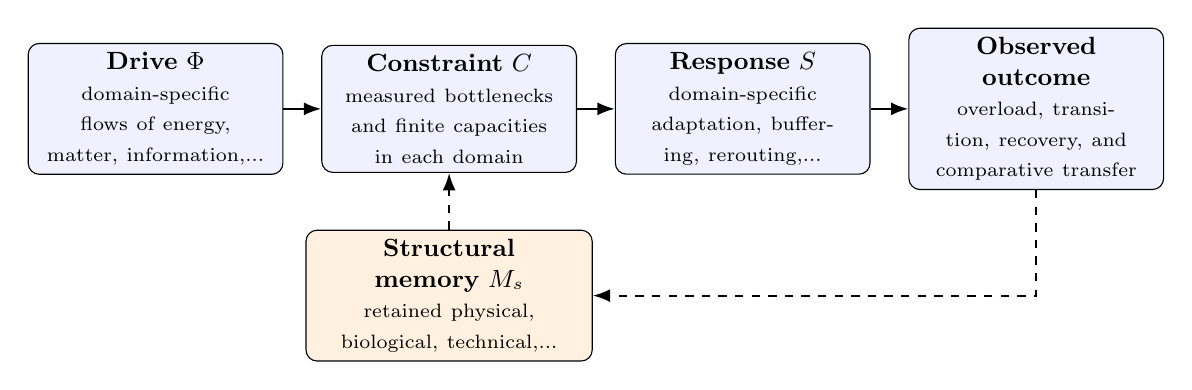
\begin{tikzpicture}[
    node distance=0.48cm,
    every node/.style={font=\small},
    box/.style={draw, rounded corners, align=center, minimum height=1.45cm, text width=3.0cm, fill=blue!6},
    memory/.style={draw, rounded corners, align=center, minimum height=1.25cm, text width=3.4cm, fill=orange!12},
    flow/.style={-{Latex[length=2.2mm]}, thick},
    feedback/.style={-{Latex[length=2.2mm]}, thick, dashed}
]
\node[box] (drive) {\textbf{Drive $\Phi$}\\\scriptsize domain-specific flows of energy, matter, information,...};
\node[box, right=of drive] (constraint) {\textbf{Constraint $C$}\\\scriptsize measured bottlenecks and finite capacities in each domain};
\node[box, right=of constraint] (response) {\textbf{Response $S$}\\\scriptsize domain-specific adaptation, buffering, rerouting,...};
\node[box, right=of response] (outcome) {\textbf{Observed outcome}\\\scriptsize overload, transition, recovery, and comparative transfer};
\node[memory, below=0.72cm of constraint] (memory) {\textbf{Structural memory $M_s$}\\\scriptsize retained physical, biological, technical,...};
\draw[flow] (drive) -- (constraint);
\draw[flow] (constraint) -- (response);
\draw[flow] (response) -- (outcome);
\draw[feedback] (outcome.south) |- (memory.east);
\draw[feedback] (memory.north) -- (constraint.south);
\end{tikzpicture}
\caption{Paper E-01 observable CDFD/AFL architecture for Universal AFL Synthesis. Solid arrows give the proposed forward chain; dashed arrows make history-dependent feedback explicit.}
\label{fig:e01-architecture}
\end{figure}

\subsection{Paper-Specific Causal Hypothesis}

For this paper, the hypothesized causal sequence is specific. A change in
domain-specific flows of energy, matter, information, organisms, capital, and force arrives faster than domain-specific adaptation, buffering, rerouting, repair, and control can compensate.
This raises or redistributes measured bottlenecks and finite capacities in each domain. If the load persists,
the retained state encoded by retained physical, biological, technical, institutional, or cognitive state changes the next response, so a later event of equal
magnitude can produce a different trajectory in overload, transition, recovery, and comparative transfer. The
scientific task is to estimate that sequence against the best ordinary model of
the domain, not merely to redescribe the outcome after it occurs.

\subsection{Cross-Scale Translation Without Mechanistic Erasure}

For the cross-domain synthesis family, the shared object is not a substance or a single physical mechanism. It is a candidate model architecture: driven flow meets finite constraint, response changes effective capacity, and retained state changes later trajectories. The architecture survives only where normalization and comparison remain meaningful. \cite{BarabasiAlbert1999,WattsStrogatz1998,Holling1973,Turing1952,Shannon1948,BakTangWiesenfeld1987}
The required scale declaration for this paper is microseconds to geological time; local components to coupled global systems. At short
scales, the key question is whether the incoming drive is transmitted,
buffered, or diverted. At intermediate scales, response changes effective
capacity and network exposure. At long scales, retained structure can alter the
state space itself. A result is genuinely cross-scale only when the aggregation
rule is stated and the same conclusion is not an artifact of averaging.

\subsection{Evidence Ladder and Discriminating Tests}

\begin{table}[htbp]
\centering
\small
\caption{Evidence ladder for Paper E-01. Each rung can fail independently.}
\begin{tabularx}{\textwidth}{|p{0.17\textwidth}|X|X|}
\hline
\textbf{Test} & \textbf{Design} & \textbf{Discriminating result} \\
\hline
Proxy audit & Measure standardized domain datasets, perturbation records, null models, and runtime diagnostics and preregister how each record maps to $\Phi$, $C$, $S$, $M_s$, and $Y$. & The mapping fails if proxies are non-identifiable, circular, or change meaning across cases. \\
\hline
Load ramp & Apply or observe matched perturbations across carefully normalized domain systems while estimating the dominant constraint and response time. & A threshold claim requires a reproducible nonlinear change and uncertainty bounds, not a visually chosen breakpoint. \\
\hline
Recovery and memory & Match present load across units with different histories, then compare recovery paths. & The memory claim requires history-dependent divergence after current conditions are controlled. \\
\hline
Model comparison & Compare the baseline domain model with and without the CDFD/AFL state variables using held-out data. & The paper's stated falsifier is: the shared architecture fails to improve prediction or comparison beyond domain baselines. \\
\hline
\end{tabularx}
\end{table}

\subsection{Research Programme and Boundary Conditions}

The immediate research programme has four steps. First, construct a documented
dataset from standardized domain datasets, perturbation records, null models, and runtime diagnostics and retain raw units before normalization.
Second, fit a baseline domain model and report its calibration and out-of-sample
error. Third, add the smallest identifiable CDFD/AFL state extension and test
whether it improves prediction of overload, transition, recovery, and comparative transfer. Fourth, repeat the
analysis across the declared scale range and publish negative cases as part of
the cross-domain translation audit.

\begin{figure}[htbp]
\centering

\includegraphics[width=0.96\textwidth]{Part_E_Synthesis/figures/universal_cascade.png}
\caption{Release-local network-cascade stress test generated by the current CDFD Runtime. The figure is a numerical diagnostic, not field validation of a domain claim.}
\label{fig:e01-runtime-cascade}
\end{figure}

\begin{figure}[htbp]
\centering

\includegraphics[width=0.96\textwidth]{Part_E_Synthesis/figures/domain_sweep_psi.png}
\caption{Selected-domain adapter sweep generated from the release-local Part IV discovery pass. Differences show the declared adapter parameterization and provide targets for later calibration.}
\label{fig:e01-domain-sweep}
\end{figure}
% END PART IV MAJOR CROSS-DOMAIN UPGRADE

\section{Conclusion}

Part IV presents a single cross-domain modelling language. Its value depends on
whether that language produces clearer measurable hypotheses than analogy alone.
The release therefore keeps claim status, reproducibility, and falsification
standards visible beside the manuscripts and outputs.

\section*{Conflict of Interest}
The author declares no conflict of interest.

\section*{Data Availability}
Part-specific runtime diagnostics are under each Part's \path{outputs/} directory.

Release-wide code: \path{Part_E_Synthesis/supplementary/}.

Generated summaries: \path{Part_E_Synthesis/outputs/}.

Figures: \path{Part_E_Synthesis/figures/}.


\section{Reference Layer}
\bibliographystyle{plain}
\bibliography{universal_afl_references}
\end{document}
